%% bare_jrnl.tex
%% V1.4b
%% 2015/08/26
%% by Michael Shell
%% see http://www.michaelshell.org/
%% for current contact information.
%%
%% This is a skeleton file demonstrating the use of IEEEtran.cls
%% (requires IEEEtran.cls version 1.8b or later) with an IEEE
%% journal paper.
%%
%% Support sites:
%% http://www.michaelshell.org/tex/ieeetran/
%% http://www.ctan.org/pkg/ieeetran
%% and
%% http://www.ieee.org/

%%*************************************************************************
%% Legal Notice:
%% This code is offered as-is without any warranty either expressed or
%% implied; without even the implied warranty of MERCHANTABILITY or
%% FITNESS FOR A PARTICULAR PURPOSE!
%% User assumes all risk.
%% In no event shall the IEEE or any contributor to this code be liable for
%% any damages or losses, including, but not limited to, incidental,
%% consequential, or any other damages, resulting from the use or misuse
%% of any information contained here.
%%
%% All comments are the opinions of their respective authors and are not
%% necessarily endorsed by the IEEE.
%%
%% This work is distributed under the LaTeX Project Public License (LPPL)
%% ( http://www.latex-project.org/ ) version 1.3, and may be freely used,
%% distributed and modified. A copy of the LPPL, version 1.3, is included
%% in the base LaTeX documentation of all distributions of LaTeX released
%% 2003/12/01 or later.
%% Retain all contribution notices and credits.
%% ** Modified files should be clearly indicated as such, including  **
%% ** renaming them and changing author support contact information. **
%%*************************************************************************


% *** Authors should verify (and, if needed, correct) their LaTeX system  ***
% *** with the testflow diagnostic prior to trusting their LaTeX platform ***
% *** with production work. The IEEE's font choices and paper sizes can   ***
% *** trigger bugs that do not appear when using other class files.       ***                          ***
% The testflow support page is at:
% http://www.michaelshell.org/tex/testflow/



\documentclass[journal]{IEEEtran}
%
% If IEEEtran.cls has not been installed into the LaTeX system files,
% manually specify the path to it like:
% \documentclass[journal]{../sty/IEEEtran}





% Some very useful LaTeX packages include:
% (uncomment the ones you want to load)


% *** MISC UTILITY PACKAGES ***
%
%\usepackage{ifpdf}
% Heiko Oberdiek's ifpdf.sty is very useful if you need conditional
% compilation based on whether the output is pdf or dvi.
% usage:
% \ifpdf
%   % pdf code
% \else
%   % dvi code
% \fi
% The latest version of ifpdf.sty can be obtained from:
% http://www.ctan.org/pkg/ifpdf
% Also, note that IEEEtran.cls V1.7 and later provides a builtin
% \ifCLASSINFOpdf conditional that works the same way.
% When switching from latex to pdflatex and vice-versa, the compiler may
% have to be run twice to clear warning/error messages.






% *** CITATION PACKAGES ***
%
% *** CITATION PACKAGES ***
%
\usepackage{amsmath}
\usepackage{amssymb}
\usepackage{bm}
\usepackage{cite}
\usepackage{graphicx}
\usepackage{multirow}
\usepackage{booktabs}
%\usepackage{cite}
% cite.sty was written by Donald Arseneau
% V1.6 and later of IEEEtran pre-defines the format of the cite.sty package
% \cite{} output to follow that of the IEEE. Loading the cite package will
% result in citation numbers being automatically sorted and properly
% "compressed/ranged". e.g., [1], [9], [2], [7], [5], [6] without using
% cite.sty will become [1], [2], [5]--[7], [9] using cite.sty. cite.sty's
% \cite will automatically add leading space, if needed. Use cite.sty's
% noadjust option (cite.sty V3.8 and later) if you want to turn this off
% such as if a citation ever needs to be enclosed in parenthesis.
% cite.sty is already installed on most LaTeX systems. Be sure and use
% version 5.0 (2009-03-20) and later if using hyperref.sty.
% The latest version can be obtained at:
% http://www.ctan.org/pkg/cite
% The documentation is contained in the cite.sty file itself.






% *** GRAPHICS RELATED PACKAGES ***
%
\ifCLASSINFOpdf
  % \usepackage[pdftex]{graphicx}
  % declare the path(s) where your graphic files are
  % \graphicspath{{../pdf/}{../jpeg/}}
  % and their extensions so you won't have to specify these with
  % every instance of \includegraphics
  % \DeclareGraphicsExtensions{.pdf,.jpeg,.png}
\else
  % or other class option (dvipsone, dvipdf, if not using dvips). graphicx
  % will default to the driver specified in the system graphics.cfg if no
  % driver is specified.
  % \usepackage[dvips]{graphicx}
  % declare the path(s) where your graphic files are
  % \graphicspath{{../eps/}}
  % and their extensions so you won't have to specify these with
  % every instance of \includegraphics
  % \DeclareGraphicsExtensions{.eps}
\fi
% graphicx was written by David Carlisle and Sebastian Rahtz. It is
% required if you want graphics, photos, etc. graphicx.sty is already
% installed on most LaTeX systems. The latest version and documentation
% can be obtained at:
% http://www.ctan.org/pkg/graphicx
% Another good source of documentation is "Using Imported Graphics in
% LaTeX2e" by Keith Reckdahl which can be found at:
% http://www.ctan.org/pkg/epslatex
%
% latex, and pdflatex in dvi mode, support graphics in encapsulated
% postscript (.eps) format. pdflatex in pdf mode supports graphics
% in .pdf, .jpeg, .png and .mps (metapost) formats. Users should ensure
% that all non-photo figures use a vector format (.eps, .pdf, .mps) and
% not a bitmapped formats (.jpeg, .png). The IEEE frowns on bitmapped formats
% which can result in "jaggedy"/blurry rendering of lines and letters as
% well as large increases in file sizes.
%
% You can find documentation about the pdfTeX application at:
% http://www.tug.org/applications/pdftex





% *** MATH PACKAGES ***
%
%\usepackage{amsmath}
% A popular package from the American Mathematical Society that provides
% many useful and powerful commands for dealing with mathematics.
%
% Note that the amsmath package sets \interdisplaylinepenalty to 10000
% thus preventing page breaks from occurring within multiline equations. Use:
%\interdisplaylinepenalty=2500
% after loading amsmath to restore such page breaks as IEEEtran.cls normally
% does. amsmath.sty is already installed on most LaTeX systems. The latest
% version and documentation can be obtained at:
% http://www.ctan.org/pkg/amsmath





% *** SPECIALIZED LIST PACKAGES ***
%
%\usepackage{algorithmic}
% algorithmic.sty was written by Peter Williams and Rogerio Brito.
% This package provides an algorithmic environment fo describing algorithms.
% You can use the algorithmic environment in-text or within a figure
% environment to provide for a floating algorithm. Do NOT use the algorithm
% floating environment provided by algorithm.sty (by the same authors) or
% algorithm2e.sty (by Christophe Fiorio) as the IEEE does not use dedicated
% algorithm float types and packages that provide these will not provide
% correct IEEE style captions. The latest version and documentation of
% algorithmic.sty can be obtained at:
% http://www.ctan.org/pkg/algorithms
% Also of interest may be the (relatively newer and more customizable)
% algorithmicx.sty package by Szasz Janos:
% http://www.ctan.org/pkg/algorithmicx




% *** ALIGNMENT PACKAGES ***
%
%\usepackage{array}
% Frank Mittelbach's and David Carlisle's array.sty patches and improves
% the standard LaTeX2e array and tabular environments to provide better
% appearance and additional user controls. As the default LaTeX2e table
% generation code is lacking to the point of almost being broken with
% respect to the quality of the end results, all users are strongly
% advised to use an enhanced (at the very least that provided by array.sty)
% set of table tools. array.sty is already installed on most systems. The
% latest version and documentation can be obtained at:
% http://www.ctan.org/pkg/array


% IEEEtran contains the IEEEeqnarray family of commands that can be used to
% generate multiline equations as well as matrices, tables, etc., of high
% quality.




% *** SUBFIGURE PACKAGES ***
%\ifCLASSOPTIONcompsoc
%  \usepackage[caption=false,font=normalsize,labelfont=sf,textfont=sf]{subfig}
%\else
%  \usepackage[caption=false,font=footnotesize]{subfig}
%\fi
% subfig.sty, written by Steven Douglas Cochran, is the modern replacement
% for subfigure.sty, the latter of which is no longer maintained and is
% incompatible with some LaTeX packages including fixltx2e. However,
% subfig.sty requires and automatically loads Axel Sommerfeldt's caption.sty
% which will override IEEEtran.cls' handling of captions and this will result
% in non-IEEE style figure/table captions. To prevent this problem, be sure
% and invoke subfig.sty's "caption=false" package option (available since
% subfig.sty version 1.3, 2005/06/28) as this is will preserve IEEEtran.cls
% handling of captions.
% Note that the Computer Society format requires a larger sans serif font
% than the serif footnote size font used in traditional IEEE formatting
% and thus the need to invoke different subfig.sty package options depending
% on whether compsoc mode has been enabled.
%
% The latest version and documentation of subfig.sty can be obtained at:
% http://www.ctan.org/pkg/subfig




% *** FLOAT PACKAGES ***
%
%\usepackage{fixltx2e}
% fixltx2e, the successor to the earlier fix2col.sty, was written by
% Frank Mittelbach and David Carlisle. This package corrects a few problems
% in the LaTeX2e kernel, the most notable of which is that in current
% LaTeX2e releases, the ordering of single and double column floats is not
% guaranteed to be preserved. Thus, an unpatched LaTeX2e can allow a
% single column figure to be placed prior to an earlier double column
% figure.
% Be aware that LaTeX2e kernels dated 2015 and later have fixltx2e.sty's
% corrections already built into the system in which case a warning will
% be issued if an attempt is made to load fixltx2e.sty as it is no longer
% needed.
% The latest version and documentation can be found at:
% http://www.ctan.org/pkg/fixltx2e


%\usepackage{stfloats}
% stfloats.sty was written by Sigitas Tolusis. This package gives LaTeX2e
% the ability to do double column floats at the bottom of the page as well
% as the top. (e.g., "\begin{figure*}[!b]" is not normally possible in
% LaTeX2e). It also provides a command:
%\fnbelowfloat
% to enable the placement of footnotes below bottom floats (the standard
% LaTeX2e kernel puts them above bottom floats). This is an invasive package
% which rewrites many portions of the LaTeX2e float routines. It may not work
% with other packages that modify the LaTeX2e float routines. The latest
% version and documentation can be obtained at:
% http://www.ctan.org/pkg/stfloats
% Do not use the stfloats baselinefloat ability as the IEEE does not allow
% \baselineskip to stretch. Authors submitting work to the IEEE should note
% that the IEEE rarely uses double column equations and that authors should try
% to avoid such use. Do not be tempted to use the cuted.sty or midfloat.sty
% packages (also by Sigitas Tolusis) as the IEEE does not format its papers in
% such ways.
% Do not attempt to use stfloats with fixltx2e as they are incompatible.
% Instead, use Morten Hogholm'a dblfloatfix which combines the features
% of both fixltx2e and stfloats:
%
% \usepackage{dblfloatfix}
% The latest version can be found at:
% http://www.ctan.org/pkg/dblfloatfix




%\ifCLASSOPTIONcaptionsoff
%  \usepackage[nomarkers]{endfloat}
% \let\MYoriglatexcaption\caption
% \renewcommand{\caption}[2][\relax]{\MYoriglatexcaption[#2]{#2}}
%\fi
% endfloat.sty was written by James Darrell McCauley, Jeff Goldberg and
% Axel Sommerfeldt. This package may be useful when used in conjunction with
% IEEEtran.cls'  captionsoff option. Some IEEE journals/societies require that
% submissions have lists of figures/tables at the end of the paper and that
% figures/tables without any captions are placed on a page by themselves at
% the end of the document. If needed, the draftcls IEEEtran class option or
% \CLASSINPUTbaselinestretch interface can be used to increase the line
% spacing as well. Be sure and use the nomarkers option of endfloat to
% prevent endfloat from "marking" where the figures would have been placed
% in the text. The two hack lines of code above are a slight modification of
% that suggested by in the endfloat docs (section 8.4.1) to ensure that
% the full captions always appear in the list of figures/tables - even if
% the user used the short optional argument of \caption[]{}.
% IEEE papers do not typically make use of \caption[]'s optional argument,
% so this should not be an issue. A similar trick can be used to disable
% captions of packages such as subfig.sty that lack options to turn off
% the subcaptions:
% For subfig.sty:
% \let\MYorigsubfloat\subfloat
% \renewcommand{\subfloat}[2][\relax]{\MYorigsubfloat[]{#2}}
% However, the above trick will not work if both optional arguments of
% the \subfloat command are used. Furthermore, there needs to be a
% description of each subfigure *somewhere* and endfloat does not add
% subfigure captions to its list of figures. Thus, the best approach is to
% avoid the use of subfigure captions (many IEEE journals avoid them anyway)
% and instead reference/explain all the subfigures within the main caption.
% The latest version of endfloat.sty and its documentation can obtained at:
% http://www.ctan.org/pkg/endfloat
%
% The IEEEtran \ifCLASSOPTIONcaptionsoff conditional can also be used
% later in the document, say, to conditionally put the References on a
% page by themselves.




% *** PDF, URL AND HYPERLINK PACKAGES ***
%
%\usepackage{url}
% url.sty was written by Donald Arseneau. It provides better support for
% handling and breaking URLs. url.sty is already installed on most LaTeX
% systems. The latest version and documentation can be obtained at:
% http://www.ctan.org/pkg/url
% Basically, \url{my_url_here}.

\newcommand{\argmax}{\mathop{\rm arg\ max}\limits}


% *** Do not adjust lengths that control margins, column widths, etc. ***
% *** Do not use packages that alter fonts (such as pslatex).         ***
% There should be no need to do such things with IEEEtran.cls V1.6 and later.
% (Unless specifically asked to do so by the journal or conference you plan
% to submit to, of course. )


% correct bad hyphenation here
\hyphenation{op-tical net-works semi-conduc-tor}


\begin{document}
%
% paper title
% Titles are generally capitalized except for words such as a, an, and, as,
% at, but, by, for, in, nor, of, on, or, the, to and up, which are usually
% not capitalized unless they are the first or last word of the title.
% Linebreaks \\ can be used within to get better formatting as desired.
% Do not put math or special symbols in the title.
\title{An EEG Analysis Method Based on a Multivariate Scale Mixture Model and Related Application to Epileptic Seizure Detection}
%
%
% author names and IEEE memberships
% note positions of commas and nonbreaking spaces ( ~ ) LaTeX will not break
% a structure at a ~ so this keeps an author's name from being broken across
% two lines.
% use \thanks{} to gain access to the first footnote area
% a separate \thanks must be used for each paragraph as LaTeX2e's \thanks
% was not built to handle multiple paragraphs
%

\author{Ryota~Onishi,
        Akira~Furui,~\IEEEmembership{Member,~IEEE,}
        Akihito~Takeuchi,
        Tomoyuki~Akiyama,
        and~Toshio~Tsuji${}^{*}$,~\IEEEmembership{Member,~IEEE}% <-this % stops a space
\thanks{R.~Onishi, A.~Furui and ${}^{*}$T.~Tsuji are with the Graduate School of Engineering,Hiroshima University, Higashi-hiroshima, 739-8527 Japan (e-mail: ryotaonishi@hiroshima-u.ac.jp; tsuji@bsys.hiroshima-u.ac.jp).}% <-this % stops a space
\thanks{A.~Takeuchi is with the Department of Neonatology, Okayama Medical Center, National Hospital Organaization.}
\thanks{T.~Akiyama is with the Department of Child Neurology, Okayama University Hospital.}% <-this % stops a space
\thanks{Manuscript received April 19, 2005; revised August 26, 2015.}}
% note the % following the last \IEEEmembership and also \thanks -
% these prevent an unwanted space from occurring between the last author name
% and the end of the author line. i.e., if you had this:
%
% \author{....lastname \thanks{...} \thanks{...} }
%                     ^------------^------------^----Do not want these spaces!
%
% a space would be appended to the last name and could cause every name on that
% line to be shifted left slightly. This is one of those "LaTeX things". For
% instance, "\textbf{A} \textbf{B}" will typeset as "A B" not "AB". To get
% "AB" then you have to do: "\textbf{A}\textbf{B}"
% \thanks is no different in this regard, so shield the last } of each \thanks
% that ends a line with a % and do not let a space in before the next \thanks.
% Spaces after \IEEEmembership other than the last one are OK (and needed) as
% you are supposed to have spaces between the names. For what it is worth,
% this is a minor point as most people would not even notice if the said evil
% space somehow managed to creep in.



% The paper headers
\markboth{Journal of \LaTeX\ Class Files,~Vol.~14, No.~8, August~2015}%
{Shell \MakeLowercase{\textit{et al.}}: Bare Demo of IEEEtran.cls for IEEE Journals}
% The only time the second header will appear is for the odd numbered pages
% after the title page when using the twoside option.
%
% *** Note that you probably will NOT want to include the author's ***
% *** name in the headers of peer review papers.                   ***
% You can use \ifCLASSOPTIONpeerreview for conditional compilation here if
% you desire.




% If you want to put a publisher's ID mark on the page you can do it like
% this:
%\IEEEpubid{0000--0000/00\$00.00~\copyright~2015 IEEE}
% Remember, if you use this you must call \IEEEpubidadjcol in the second
% column for its text to clear the IEEEpubid mark.



% use for special paper notices
%\IEEEspecialpapernotice{(Invited Paper)}




% make the title area
\maketitle

% As a general rule, do not put math, special symbols or citations
% in the abstract or keywords.
\begin{abstract}
\textit{Objective:}
The detection of epileptic seizures in surface electroencephalogram (EEG) signals is an important problem in biomedical engineering.
This paper proposes multichannel EEG analysis method based on a multivariate scale mixture model (MVSMM) that can be evaluated Gaussianity and non-Gaussianity by one dimensional parameter.
\textit{Methods:}
In the model, a surface EEG signals at a certain time follows a multivariate Gaussian distribution, and its variance-covariance matrix is handled as a random variable that follows an inverse Wishart distribution.
Thereby, we obtain by summing an infinite number of multivariate Gaussian distributions having different variance-covariance matrices.
The proposed method combines a MVSMM with a filter bank, thereby allowing the time-series estimation of stochastic fluctuations latent in each frequency band of EEG.
In addition, we introduce the index representing stochastic fluctuations based on MVSMM parameter.
%In this paper, we describe the formulation of a non-Gaussian EMG model based on a scale mixture distribution. In the model, an EMG signal at a certain time follows a Gaussian distribution, and its variance is handled as a random variable that follows an inverse gamma distribution. Accordingly, the probability distribution of EMG signals is assumed to be a mixture of Gaussians with the same mean but different variances. The EMG variance distribution is estimated via marginal likelihood maximization.
\textit{Results:}
We applied the proposed method to the multichannel EEG data from twenty patients with focal epilepsy. The results demonstrated that the proposed index was significantly increased during epileptic seizures, especially in high frequency band. The index calculated in the high frequency band provided a higher classification performance between seizure segments and non-seizure segments (AUC = 0.881), which was significantly higher than the conventional amplitude-based index.
\textit{Conclusion:}
This study proposed a multivariate scale mixture distribution-based stochastic EEG model capable of representing stochastic fluctuations associated with epileptic seizures.
In high frequency band, proposed index shows the possibility of clasification of epileptic seizures.
\textit{Significance:}
The proposed model can be used in various fields of EEG, and helps to characterize stochastic fluctuations of multichannel EEG signals.

%In the experiment, we estimate parameters using artificially generated signals, and evaluate the estimated accuracy. we describe proposed model validity to estimate parameter and fit to  recorded EEGs from twenty patients.

\end{abstract}

% Note that keywords are not normally used for peerreview papers.
\begin{IEEEkeywords}
Electroencephalogram (EEG), stochastic model, stochastic fluctuations, multivariate scale mixture model, epileptic seizures, non-Gaussianity.
\end{IEEEkeywords}






% For peer review papers, you can put extra information on the cover
% page as needed:
% \ifCLASSOPTIONpeerreview
% \begin{center} \bfseries EDICS Category: 3-BBND \end{center}
% \fi
%
% For peerreview papers, this IEEEtran command inserts a page break and
% creates the second title. It will be ignored for other modes.
\IEEEpeerreviewmaketitle



\section{Introduction}
% The very first letter is a 2 line initial drop letter followed
% by the rest of the first word in caps.
%
% form to use if the first word consists of a single letter:
% \IEEEPARstart{A}{demo} file is ....
%
% form to use if you need the single drop letter followed by
% normal text (unknown if ever used by the IEEE):
% \IEEEPARstart{A}{}demo file is ....
%
% Some journals put the first two words in caps:
% \IEEEPARstart{T}{his demo} file is ....
%
% Here we have the typical use of a "T" for an initial drop letter
% and "HIS" in caps to complete the first word.
\IEEEPARstart{E}{pilepsy} is a neurological disorder that causes epileptic seizures due to abnormalities in cranial nerves, and it is reported that there are around 50 million patients worldwide~\cite{WHO}.てんかん発作を放置することは脳障害の増大に繋がる可能性があることから,発作の早期発見が重要である.しかしながら,てんかん発作の診断には多くの専門知識や経験が求められるのに加え,てんかん発作は一度だけでなく反復して生じる場合がある~\cite{Kandel2000}.そのため,診断そのものにも長時間を要することから,専門医への負担が問題となっている.

従来,医師の負担軽減のため,頭皮表面から計測可能な生体電気信号である脳波(electroencephalogram : EEG)を用いて,てんかん発作を検出する方法がさまざま提案されてきた~\cite{Deburchgraeve2008,Subasi2005,kellaway1979precise,Panzica1999,fusco1993ictal,Acir2005,Greene2008}.
例えばDeburchgraeveらは,発作時における振幅の急峻な変化や高振幅の徐波の周期性に着目した脳波解析により,てんかん発作の検出を行なった~\cite{Deburchgraeve2008}.また,Subasiらはウェーブレット変換を用いて周波数解析を行なうことで,発作の有無の識別を実現している~\cite{Subasi2005}.
しかし,てんかん発作時の脳波には年齢やてんかんの種類に起因する大きな個人差が存在するため,振幅の大小や周波数の変化のみの評価では検出困難な場合があるという問題が存在した.

一方,振幅や周波数に依存しない特徴として,脳波の確率分布形状に関する研究も従来から行なわれてきた~\cite{Sounders1963,Gonen2012,Campbell1967,Weiss1973,Nurujjaman2009,Charles1999}.
古くは脳波を定常なガウス分布であると仮定することが一般的であったが~\cite{Sounders1963,Gonen2012},Campbellらによって脳波が非ガウスな性質を持つことが統計的に示されたことで~\cite{Campbell1967},脳波のガウス性に着目した解析がさまざま行なわれるようになった~\cite{Gonen2012,Weiss1973,Nurujjaman2009,Charles1999}.
てんかん発作と脳波のガウス性との関係に関する従来研究は少ないものの,NurujjamanらやCharlesらによっててんかん発作時の脳波が非ガウスな分布に従うことが報告されている~\cite{Nurujjaman2009,Charles1999}.
しかしながら,これらは実験的な報告に留まっており,脳波の非ガウス性を定量的に扱うための理論的な枠組みは存在しなかった.

そこで本論文では,脳波の非ガウス性が振幅の確率的変動によって生じると仮定し,尺度混合モデルに基づき,この変動を推定可能な指標を提案する.
尺度混合モデルにおいて,頭皮表面の多チャネル電極から計測された脳波を多変量ガウス分布,
そしてその分散共分散行列を逆ウィシャート分布に従う確率変数として扱う.
これにより,脳波の振幅に相当する分散共分散行列の確率的変動を評価可能である.
さらに,このモデルをフィルタバンクと組み合わせることで,脳波の各周波数帯域に潜在する
確率的変動を時系列に推定可能な解析手法へと展開する.
シミュレーション実験では,人工データに対して提案法に基づくパラメータ推定を行ない,条件を変更させた際の真値と推定値との誤差について議論する.
解析実験では,てんかん発作時の脳波に対して提案法に基づく解析を行ない,
提案モデルの適合度を検証し,推定された脳波の確率的変動と医師による診断結果との対応について議論する.

The reminder of this paper is organized as follows: Section II outlines the structure of the multivariate scale mixture model (MVSMM), the parameter estimation method, and EEG analysis method considering frequency charastalistic. Section III details the simulation experiments and  epileptic EEG analysis experiments. Section IV presents the results of these experiments, and Section V provides related discussion. Finally, Section VI states the conclusions to this study.
% You must have at least 2 lines in the paragraph with the drop letter
% (should never be an issue)

\section{Methods}

\subsection{Multivariate Scale Mixture Model of Surface EEG Signals}
Fig. \ref{fig:model} shows the stochastic relationship between the EEG signals.
In the proposed model, recorded EEG signals with $D$ electrodes $\mathbf{x} \in \mathbb{R}^{D}$ and its variance-covariance matrix $\mathbf{\Sigma} \in \mathbb{R}^{D \times D}$ as a graphical model.
$\mathbf{x}$ is handled as a random variable that follows a multivariate Gaussian distribution with a mean of zero and a variance-covariance matrix of $\mathbf{\Sigma}$.
The variance-covariance matrix  is also a random variable for which the distribution is determined by the degrees of freedom parameter $\nu \in \mathbb{R}^+$ and the scale matrix parameter $\mathbf{\Psi} \in \mathbb{R}^{D \times D}$.

%1Note that the frequency components of EMG signals are ignored in the model; only their variance is considered.

%%%%%%%%%%%%%%%%%%%%%%%%%%%%%%%%
\begin{figure}[!t]
\centering
\includegraphics[width=1.0\hsize]{figure/fig1_ver2.eps}
%\end{center}
\caption{Graphical representation of the stochastic relationship between EEG signals  and its variance-covariance matrix.
The white nodes are random variables and the black nodes are parameters to be estimated.
In the model, EEG signals $\mathbf{x} \in \mathbb{R}^{D}$ are handled as a random variable that follows a multivariate Gaussian distribution with a mean vector of $\mathbf{0}$.
The EEG variance-covariance matrix $\mathbf{\Sigma} \in \mathbb{R}^{D \times D}$ is also a random variable that follows the inverse Wishart distribution determined by the degrees of freedom parameter $\nu \in \mathbb{R}^+$ and the scale matrix $\mathbf{\Psi} \in \mathbb{R}^{D \times D}$. The parameter $\nu$ represents stochastic fluctuations of EEG signals.
The variance-covariance matrix distribution parameters are estimated via marginal likelihood maximization from recorded EEG signals.}
\label{fig:model}
\end{figure}
%%%%%%%%%%%%%%%%%%%%%%%%%%%%%%%%
First, the conditional distribution of  EEG signals $\mathbf{x}$ given $\mathbf{\Sigma}$ is expressed via the following multivariate Gaussian distribution with mean of zero:

\begin{align}
	p(\mathbf{x}|{\mathbf{\Sigma}}) &= {\mathcal N}(\mathbf{x}|{\mathbf{\Sigma}}) \nonumber\\
&= \frac{1}{(2\pi)^{D/2} |\mathbf{\Sigma}|^{1/2}} \mathrm{exp} \left[-\frac{1}{2}\mathbf{x}^\mathrm{T} {\mathbf{\Sigma}}^{-1} \mathbf{x}\right]. \label{eq:gauss_x} %eq1
\end{align}

The distribution of the variance-covariance matrix is assumed to obey an inverse Wishart distribution ${\mathcal {IW}}(\mathbf{\Sigma}; \nu, \mathbf{\Psi})$, which is known as a conjugate prior for the variance-covariance matrix of a multivariate Gaussian distribution:
%
\begin{align}
	p(\mathbf{\Sigma}) &= {\mathcal {IW}}(\mathbf{\Sigma};\nu,\mathbf{\Psi}) \nonumber\\
&= \frac{|\mathbf{\Psi}|^{\frac{\nu}{2}}}{2^{\frac{\nu D}{2}} \Gamma_D \left(\frac{\nu}{2}\right)} |\mathbf{\Sigma}|^{-\frac{\nu+D+1}{2}} \mathrm{exp} \left[-\frac{\mathrm{tr}(\mathbf{\Psi} \mathbf{\Sigma}^{-1})}{2}\right],\label{eq:p_sigma} %eq2
\end{align}
%
where $\nu$ and $\mathbf{\Psi}$ determine the inverse Wishart distribution, and are referred to as the degrees of freedom parameter and the scale matrix parameter, respectively.
Considering the marginal distribution of $\mathbf{x}$, the variance-covariance matrix $\mathbf{\Sigma}$ can be integrated out as follows:

\begin{align}
	p(\mathbf{x}) &= \int p(\mathbf{\Sigma})p(\mathbf{x}|\mathbf{\Sigma}) \mathrm{d}{\mathbf{\Sigma}} \nonumber \\
		&= \int {\mathcal {IW}}(\mathbf{\Sigma}; \nu, {\mathbf{\Psi}}) {\mathcal N}(\mathbf{x}|\mathbf{\Sigma}) \mathrm{d}{\mathbf{\Sigma}} \label{eq:marginal_x} \\ %eq3
		&= \int \frac{|{\mathbf{\Psi}}|^{\frac{\nu}{2}}}{2^{\frac{\nu D}{2}} \Gamma_D \left(\frac{\nu}{2}\right)} |\mathbf{\Sigma}|^{-\frac{\nu+D+1}{2}}\mathrm{exp} \left[-\frac{\mathrm{tr}(\mathbf{\Psi} \mathbf{\Sigma}^{-1})}{2}\right] \nonumber \\
&\quad \times\frac{1}{(2\pi)^{D/2} |\mathbf{\Sigma}|^{1/2}} \mathrm{exp} \left[-\frac{1}{2}\mathbf{x}^\mathrm{T} {\mathbf{\Sigma}}^{-1} \mathbf{x}\right] \mathrm{d}{\mathbf{\Sigma}} \nonumber \\
		&= \frac{|{\mathbf{\Psi}}|^{\frac{\nu}{2}}}{2^{\frac{\nu D}{2}} (2\pi)^\frac{D}{2} \Gamma_D \left(\frac{\nu}{2}\right)} \int |\mathbf{\Sigma}|^{-\frac{\nu+D+2}{2}}\nonumber\\
&\quad \times \mathrm{exp} \left[-\frac{1}{2}\mathrm{tr}\{(\mathbf{\Psi} + \mathbf{x} \mathbf{x}^\mathrm{T})\mathbf{\Sigma}^{-1}\}\right] \mathrm{d}{\mathbf{\Sigma}} \nonumber \\
		%&=& \frac{\Gamma_D(\frac{\nu+1}{2})}{\Gamma_D(\frac{\nu-D+1}{2})} \frac{|\frac{1}{\nu-D+1} {\mathbf{\Psi}}|^{-\frac{1}{2}}}{\left[\pi(\nu-D+1)\right]^{\frac{D}{2}}} (1+\Delta)^{-\frac{\nu+1}{2}},
\label{eq:p_x}
&= \frac{\Gamma(\frac{\nu+1}{2})}{\Gamma(\frac{\nu-D+1}{2})} \frac{|\frac{1}{\nu-D+1} {\mathbf{\Psi}}|^{-\frac{1}{2}}}{\left[\pi(\nu-D+1) \right]^{\frac{D}{2}}} (1+\Delta)^{-\frac{\nu+1}{2}} ,%eq4
\end{align}
%
where $\Delta$ is the square of Mahalanobis' distance as follows:
%
\begin{align}
	\Delta &= \mathbf{x}^\mathrm{T}{\mathbf{\Psi}}^{-1}\mathbf{x}.
\end{align}
%

From (\ref{eq:gauss_x}) and (\ref{eq:marginal_x}), $p(\mathbf{x})$ is obtained by summing an infinite number of  multivariate Gaussian distributions having different variance-covariance matrices.
As stated above, it can model marginal distribution of multidimensional EEG signals by Scale mixture distribution.

\subsection{Parameter Estimation Based on Marginal Maximum Likelihood}
Let us consider the estimation of $\nu$ and $\mathbf{\Psi}$, given $N$ samples of EEG signals $\mathbf{X} = \{\mathbf{x}_n \in \mathbb{R}^{D}; n=1,2,\cdots,N \}$. The model parameters can be estimated by maximizing the marginal likelihood $p(\mathbf{X}) = \prod_{n=1}^{N} p(\mathbf{x}_n)$.

However, the maximum likelihood solution of marginal likelihood is generally complex, so it is difficult to optimize the solution analytically~\cite{t2006}.
Therefore, we conduct this optimization of $\nu$ and $\mathbf{\Psi}$ based on the Expectation-maximization (EM) algorithm~\cite{Models1998} with the introduction of latent variable.
To simplify (\ref{eq:p_x}), we defined the new parameters as:
%
\begin{align}
	\label{eq:eq6}
	\nu&= \nu' + D - 1 \\
	\label{eq:eq7}
	\mathbf{\Psi}&= \nu' \mathbf{\Psi}'.
\end{align}
The marginal distribution can be expessed as
\begin{align}%equation 8, 9
\label{eq:eq8}
p(\mathbf{x}_n) &=\int \mathcal{IW}(\mathbf{\Sigma}_n; \nu'+D-1, \nu' \mathbf{\Psi}') \mathcal{N}(\mathbf{x}_n|\mathbf{\Sigma}_n) \mathrm{d} {\mathbf{\Sigma}_n} \\
\label{eq:eq9}
&=\frac{\Gamma(\frac{\nu'+D}{2})}{\Gamma(\frac{\nu'}{2})} \frac{|{\mathbf{\Psi}'}|^{-\frac{1}{2}}}{\left(\pi \nu' \right)^{\frac{D}{2}}} \left(1+\frac{\Delta '}{\nu '} \right)^{-\frac{\nu'+D}{2}},
\end{align}
where
\begin{align}
	\Delta ' = \mathbf{x}_n^\mathrm{T} ({\mathbf{\Psi} '})^{-1} \mathbf{x}_n.
\end{align}
Equation (\ref{eq:eq9}) is equivalent to multivariate Student-$t$ distribution $\mathrm{St}(\mathbf{x}_n|\nu', \Psi')$~\cite{t2006}. %However, the EM procedure based on (\ref{eq:eq8}) involves matrix calculations because the latent variable $\mathbf{\Sigma}$ has a matrix form, resulting in a high computational cost. #191217
Accordingly, we redefine the latent variable and replace (\ref{eq:eq8}) with the following equivalent expression, thereby allowing the efficient calculation (refer to Appendix).

\begin{equation}%equation11
\label{eq:eq11}
		p(\mathbf{x}_n) = \int \mathrm{IG}(\tau_n;\nu'/2,\nu'/2) \mathcal{N}(\mathbf{x}_n|\tau_n \mathbf{\Psi}') \mathrm{d}{\tau_n},
\end{equation}
where $\tau_n$ is a new latent variable allowing inverse Gamma distribution $\mathrm{IG(\cdot)}$.
The model parameters $\nu'$ and $\mathbf{\Psi}'$ are estimated by maximizing the marginal likelihood as outlined below.

\begin{enumerate}
\setlength{\parskip}{0cm}
\setlength{\itemsep}{0cm}
\item[(i)] Initialize each parameter with the selection of arbitrary starting values.
\item[(ii)] \textit{E-step}. Calculate the expectation of the complete-data log likelihood, denoted as $Q(\nu',\mathbf{\Psi}')$.
\begin{align}%equation 12
  Q(\nu',\mathbf{\Psi}')&=\mathbb{E} \left[\ln{\prod_{n=1}^{N}\mathrm{IG}(\tau_n;\nu'/2,\nu'/2) \mathcal{N}(\mathbf{x}_n|\tau_n \mathbf{\Psi}')}\right]  \notag  \\
  &=\sum_{n=1}^{N} \biggl[-\frac{D}{2}\ln{(2\pi)}-\frac{D}{2}\mathbb{E}\left[\ln{\tau_n}\right]-\frac{1}{2}\ln{|\mathbf{\Psi}'|} \notag \\
  &\quad-\frac{1}{2}\mathbb{E}\left[\tau^{-1}_n\right]\Delta'+\frac{\nu'}{2} \ln{\frac{\nu'}{2}} - \ln{\Gamma{\left(\frac{\nu'}{2}\right)}} \notag \\
  &\quad- \left(\frac{\nu'}{2}+1\right)\mathbb{E}\left[\ln{\tau_n}\right]-\frac{\nu'}{2}\mathbb{E}\left[\tau^{-1}_n \right] \biggr],
\end{align}
where $\mathbb{E}\left[\tau^{-1}_n\right]$ and $\mathbb{E}\left[\ln{\tau_n}\right]$ are derived by calculating the posterior distribution $p(\tau_n|\mathbf{x}_n)$ of the latent variable $\tau_n$ as follows:
\begin{equation}%equation 13
\mathbb{E}\left[\tau^{-1}_n\right]=\frac{\nu'+D}{\nu'+\Delta'}
\end{equation}
\begin{eqnarray}%equation 14
&\mathbb{E}\left[\ln{\tau_n}\right]=-\ln{\mathbb{E}\left[\tau^{-1}_n\right]}+\ln{\left(\frac{\nu'}{2}\right)}-{\psi}\left(\frac{\nu'}{2}\right)\quad.
\end{eqnarray}
where $\psi(\cdot)$ is a digamma function.
\item[(iii)] \textit{M-step}. Update the parameters by maximizing $Q(\nu',\mathbf{\Psi}')$.
By setting the derivative of $Q(\nu',\mathbf{\Psi}')$ with $\mathbf{\Psi}'$ equal zero, the new scale matrix are obtained as

\begin{equation}%equation 15
{^\mathrm{new} \mathbf{\Psi}}' = \frac{1}{N} \sum_{n=1}^{N} \mathbb{E}\left[\tau^{-1}_n\right] \mathbf{x}_n \mathbf{x}_n^\mathrm{T}.
\end{equation}
Because there is no closed form expression for the degrees of freedom parameter $\nu'$, we estimates $\nu'$ by maximazing $Q(\nu',\mathbf{\Psi}')$ based on a binary search.

\begin{equation}%equation 16
{^\mathrm{new} \nu}' = \argmax_{\nu'}  Q(\nu', {^\mathrm{new} \mathbf{\Psi}}').
\end{equation}
\item[(iv)] Evaluate the log-likelihood $\ln{p(\mathbf{X})}$ and repeat steps (ii)--(iv) until the calculation converges. Finally, estimated parameters $\nu'$ and $\mathbf{\Psi}'$ transform variance-covariance matrix distribution parameters $\nu$ and $\mathbf{\Psi}$.
\end{enumerate}
Using this procedures, the parameters of the proposed model can be estimated from recorded EEG signals.
Inverse Wishart distribution parameter $\nu$ corresponds to the degrees of freedom of multivariate Student-$t$ distribution parameter, hence $\nu$ is a distribution parameter to determine Gaussianity.
In the framework of MVSMM, we consider Gaussianity changes because of stochastic fluctuations of parameter equivalent to variances.
From the above, it can be evaluated fluctuations of variance-covariance matrix by estimating $\nu$ from recorded EEG signals.

\subsection{Proposed EEG Analysis Methods}
%%%%%%%%%%%%%%%%%%%%%%%%%%%%%%%%
\begin{figure*}[!ht]
\centering
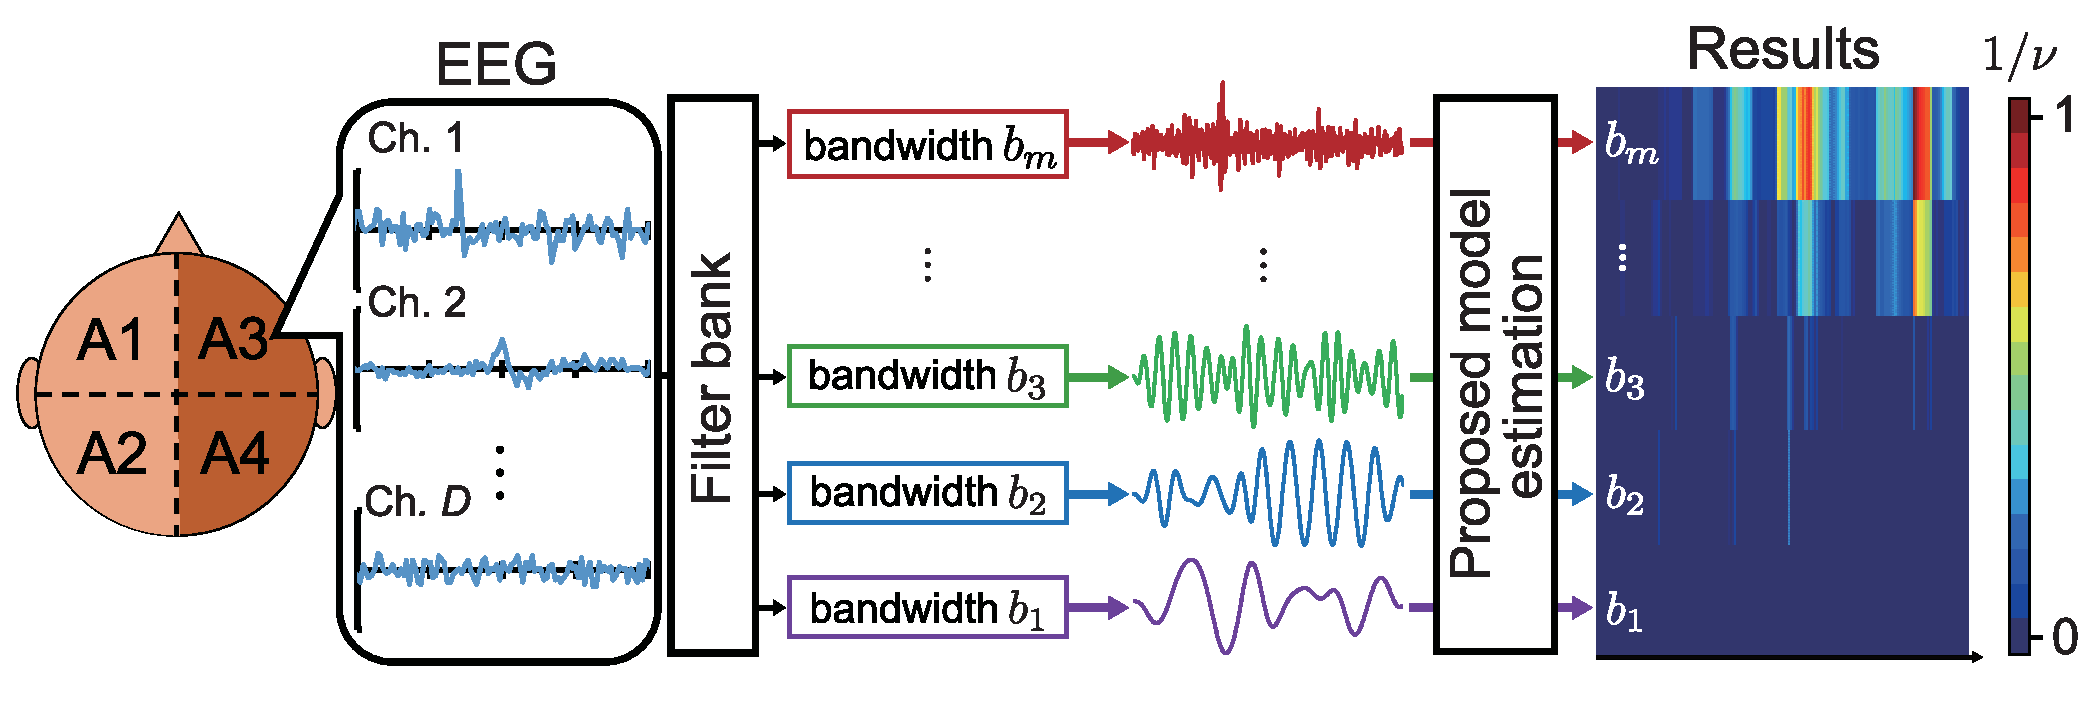
\includegraphics[width=0.95\hsize]{figure/system_3.eps}
%\end{center}
\caption{Overview of the proposed analysis method. The recorded EEG signals are decomposed into $b_1$--$b_n$ frequency band by using filterbank consisting of parallel band pass filters, then the parameter is estimated based on the proposed model and show the results by using color map.}
\label{fig:system}
\end{figure*}
%%%%%%%%%%%%%%%%%%%%%%%%%%%%%%%%
Figure \ref{fig:system} shows an overall outline of proposed analysis method. In proposed method, observed EEG signals were decomposed into multiple frequency bands by using filterbank consisting of parallel band-pass filters. Additionally, we estimate stochastic fluctuations for signals in each frequency band based on MVSMM.

まず,$D$対の電極から計測された時刻$t$における脳波を$\mathbf{x}_t \in \mathbb{R}^D$とする.そして,$\mathbf{x}_t$に対して3次のバタワースバンドパスフィルタによって構成されたフィルタバンクを適用することで,信号を$M$個の周波数帯域$b_1, \cdots, b_M$に分割し,得られた信号を$x_t^{(b_m)}$ ($m = 1,\cdots, M$)とする.
%$\delta$ (1--3 Hz), $\theta$ (4--7 Hz), $\alpha$ (8--12 Hz), $\beta$ (13--24 Hz), $\gamma$ (25--100 Hz) の5つの周波数帯域に分解し,得られた信号を$\mathbf{x}^{(b)}_t$ ($b \in\{\delta, \theta, \alpha,\beta, \gamma\}$)とする.なお,これらの周波数帯域は脳波の特性をとらえるために一般的に用いられているものである~\cite{ep1994}.
次に,$\mathbf{x}^{(b_m)}_t$に対して周波数帯域ごとに尺度混合モデルに基づく分散共分散行列分布のパラメータ推定を行ない,確率的変動を特徴づける$\nu$を取得する.ここで,脳波は時系列に特性が大きく変化する信号であるため,各帯域の信号$\mathbf{x}^{(b_m)}_t$に対してwindow length $W$ (s)のsliding windowを適用し,窓内のサンプルに対してII--\textit{B}.の手順に基づきパラメータ$\nu$を推定する.このsliding windowをsliding width $S$ (s)で連続的に推定を行なうことで,時系列に$\nu$の推定結果を取得可能である.ここで,$\nu$は$\infty$に近くなるほど分布がガウス分布に近づく,つまり確率的変動が小さくなることを意味するパラメータである.そこで本論文では,$\nu$の逆数である$1/\nu$を算出し,これを確率的変動を特徴づける指標として用いる.この$1/\nu$は,値が大きいほど脳波の確率的変動が大きいことを示す.

以上より,脳波の各帯域に潜在する確率的変動を時系列に取得することができる.
また,事前に脳波の電極配置を複数の領域に分割しておき,領域ごとに上記の解析を行なうことで,確率的変動の空間分布を取得することも可能である.

% An example of a floating figure using the graphicx package.
% Note that \label must occur AFTER (or within) \caption.
% For figures, \caption should occur after the \includegraphics.
% Note that IEEEtran v1.7 and later has special internal code that
% is designed to preserve the operation of \label within \caption
% even when the captionsoff option is in effect. However, because
% of issues like this, it may be the safest practice to put all your
% \label just after \caption rather than within \caption{}.
%
% Reminder: the "draftcls" or "draftclsnofoot", not "draft", class
% option should be used if it is desired that the figures are to be
% displayed while in draft mode.
%
%\begin{figure}[!t]
%\centering
%\includegraphics[width=2.5in]{myfigure}
% where an .eps filename suffix will be assumed under latex,
% and a .pdf suffix will be assumed for pdflatex; or what has been declared
% via \DeclareGraphicsExtensions.
%\caption{Simulation results for the network.}
%\label{fig_sim}
%\end{figure}

% Note that the IEEE typically puts floats only at the top, even when this
% results in a large percentage of a column being occupied by floats.


% An example of a double column floating figure using two subfigures.
% (The subfig.sty package must be loaded for this to work.)
% The subfigure \label commands are set within each subfloat command,
% and the \label for the overall figure must come after \caption.
% \hfil is used as a separator to get equal spacing.
% Watch out that the combined width of all the subfigures on a
% line do not exceed the text width or a line break will occur.
%
%\begin{figure*}[!t]
%\centering
%\subfloat[Case I]{\includegraphics[width=2.5in]{box}%
%\label{fig_first_case}}
%\hfil
%\subfloat[Case II]{\includegraphics[width=2.5in]{box}%
%\label{fig_second_case}}
%\caption{Simulation results for the network.}
%\label{fig_sim}
%\end{figure*}
%
% Note that often IEEE papers with subfigures do not employ subfigure
% captions (using the optional argument to \subfloat[]), but instead will
% reference/describe all of them (a), (b), etc., within the main caption.
% Be aware that for subfig.sty to generate the (a), (b), etc., subfigure
% labels, the optional argument to \subfloat must be present. If a
% subcaption is not desired, just leave its contents blank,
% e.g., \subfloat[].


% An example of a floating table. Note that, for IEEE style tables, the
% \caption command should come BEFORE the table and, given that table
% captions serve much like titles, are usually capitalized except for words
% such as a, an, and, as, at, but, by, for, in, nor, of, on, or, the, to
% and up, which are usually not capitalized unless they are the first or
% last word of the caption. Table text will default to \footnotesize as
% the IEEE normally uses this smaller font for tables.
% The \label must come after \caption as always.
%
%\begin{table}[!t]
%% increase table row spacing, adjust to taste
%\renewcommand{\arraystretch}{1.3}
% if using array.sty, it might be a good idea to tweak the value of
% \extrarowheight as needed to properly center the text within the cells
%\caption{An Example of a Table}
%\label{table_example}
%\centering
%% Some packages, such as MDW tools, offer better commands for making tables
%% than the plain LaTeX2e tabular which is used here.
%\begin{tabular}{|c||c|}
%\hline
%One & Two\\
%\hline
%Three & Four\\
%\hline
%\end{tabular}
%\end{table}


% Note that the IEEE does not put floats in the very first column
% - or typically anywhere on the first page for that matter. Also,
% in-text middle ("here") positioning is typically not used, but it
% is allowed and encouraged for Computer Society conferences (but
% not Computer Society journals). Most IEEE journals/conferences use
% top floats exclusively.
% Note that, LaTeX2e, unlike IEEE journals/conferences, places
% footnotes above bottom floats. This can be corrected via the
% \fnbelowfloat command of the stfloats package.




\section{Experiments}
%%%%%%%%%%%%%%%%%%%%%%%%%%%%%%%%
\begin{figure}[!t]
\centering
\includegraphics[width=0.6\hsize]{figure/electrodes.eps}
%\end{center}
\caption{International 10--20 electrode montage}
\label{fig:electrodes}
\end{figure}

\subsection{Simulation}
提案モデルに基づく推定の精度を検証するため,推定値と実測値の誤差率を評価するシミュレーション実験を行なった.提案モデルの周辺分布が$t$分布と等価であることを利用し,$t$分布$\mathrm{St}(\mathbf{x}_t|\nu'_0, \mathbf{\Psi}'_0)$に従う乱数系列$\{\mathbf{x}_t \in \mathbb{R}^D (t = 1, \cdots, T)\}$を生成した.ここで,$\{\mathbf{x}_t \}$はサンプリング周波数$f_s$で計測された脳波の時系列とみなされる.分布推定の精度は, (\ref{eq:eq6}), (\ref{eq:eq7})式に基づき$\nu'_0,\mathbf{\Psi}'_0$を逆ウィシャート分布のパラメータに変換し,真値$\nu_0$, $\mathbf{\Psi}_0$と推定値$\nu$, $\mathbf{\Psi}$を比較することで示す.精度の評価指標として,各パラメータに対する absolute percentage errorを,それぞれ${|\nu_0 -\nu|}/{|\nu_0|}\times100$, ${\|\mathbf{\Psi}_0-\mathbf{\Psi}\|_F}/{\|\mathbf{\Psi}_0\|_F}\times100$のように算出した.
ここで,$\|\mathbf{\Psi}\|_F$は$\mathbf{\Psi}$のフロベニウスノルム~\cite{GeneHowardGolub2013}であり,$\mathbf{\Psi}$の要素${\psi_{ij}}$を用いて次のように求まる.
\begin{align}%ディスプレイ用番号付き12
	\|\mathbf{\Psi}\|_F=\sqrt{\sum_{i=1}^D \sum_{j=1}^D |{\psi_{ij}}|^2}
\end{align}

各パラメータの推定には,信号$\{\mathbf{x}_t \}$の最初の$W$秒間の値を用いた.推定窓の長さ$W$は 1, 2, 5, 10, 15, 20, 30, 50, 100 s,次元数$D$は 1, 2, 4, 8, 16, 19と変更させた.Average absolute percentage errorは$t$分布の二つのパラメータ自由度$\nu'_0$と尺度行列$\mathbf{\Psi}'_0$を400回変更することで求めた ($\nu'_0=0.5,1.0,1.5,\cdots,10.0, {\psi'_0}_{ii} =1.0, 2.0, 3.0,\cdots, 20.0$).なお,$\mathbf{\Psi}'_0$は対角成分${\psi'_0}_{ii}$のみ変更し,非対角成分は0.5に固定した.人工データ生成における$T$と$f_s$はそれぞれ100 sと500 Hzに設定した.

\subsection{Epileptic EEG analysis}
本実験では,提案モデルの妥当性評価と提案指標である$1/\nu$の有効性の検証を行なう.
被験者は,専門医によって焦点発作を伴う焦点性てんかんと診断されたてんかん患者20名であり,仰臥位で脳波の計測を行なった.また,各被験者の情報,解析に用いた時間,および発作持続時間を Table \ref{table:conditions}に示す.The EEG was recorded with a digital sampling frequency at 500 Hz by using EEG instrument (Neurofax EEG-1218, Nihon Kohden, Tokyo, Japan). Surface electrodes ($D=19$) placed on the scalp according to the international 10--20 electrode system with reference electrodes on both earlobes: A1, A2 (refer to Fig. \ref{fig:electrodes}).
なお,本論文における解析は岡山大学生命倫理委員会の承認のもと実施した (承認番号:研1706-019).
%%%%%%%%%%%%%%%%%%%%%%%%%%%%%%%%

%=====================
%Table1 被験者
%=====================
\begin{table}[!t]
 \begin{center}
 \caption[Subject conditions]{\small Subject conditions}
 \label{table:conditions}
 \vspace{-2.5mm}
 \scalebox{1.1}[1.1]{%size
  \begin{tabular}{ccccc}
   \toprule %booktabs
   \multirow{2}{*}{Subject} &  \multirow{2}{*}{Sex} &  Age  & Total data & Seizure duration \\
   & & (year) &  length (s) & (s) \\
   \midrule %booktabs
   Sub. A & Male & 2 & 300 & 71\\ %AS
   Sub. B & Male & 23 & 300 & 54\\ %ZX
   Sub. C & Male & 2 & 300 & 71\\ %AR
   Sub. D & Male & 4 & 380 & 93\\ %IP
   Sub. E & Female & 31 & 320  & 39\\ %IQ
   Sub. F & Male & 41 & 300 & 32\\%M0 20190918
   Sub. G & Female & 3 & 240 & 53\\%62 20191209
   %Sub. F & Male & 0.5 & 500 & 158\\ %IS省くかも20190716 20190918省く!!
   %Sub. G & Female & 14 & 420 & 72\\ %IT省くかも2019071	6 20190918省く!!
   Sub. H & Male & 19 & 390 & 36\\ %IV
   Sub. I & Male & 0.8 & 360  & 98\\ %15
   Sub. J & Male & 20 & 390 & 16\\ %IW
   Sub. K & Male & 36 & 300 & 23\\ %NR
   Sub. L & Male & 9 & 300 & 43\\ %NS
   Sub. M & Male & 13 & 300  & 43\\ %ZR
   Sub. N & Male & 15 & 300 & 48\\%61 20191209
   %Sub. N & Male & 12 & 300 & 88\\ %ZS
   Sub. O & Male & 8 & 300 & 17\\ %ZT
   Sub. P & Female & 19 & 300 & 69\\ %ZV
   Sub. Q & Male & 27 & 420 & 62\\ %AB
	 Sub. R & Male & 38 & 300 & 65\\ %ZY
	 Sub. S & Male & 17 & 300 & 17\\ %ZZ
	 Sub. T & Male & 19 & 300 & 65\\ %00
   \bottomrule %booktabs
  \end{tabular}
  }
 \end{center}
\end{table}

%=====================
全被験者の計測時間すべての脳波に対して提案モデルのフィッティング,およびII.Cに基づく指標$1/\nu$の算出を行なった.
本実験では周波数帯域を$b_m \in\{\delta, \theta, \alpha,\beta, \gamma\}$とし,計測した脳波を
$\delta$ (1--3 Hz), $\theta$ (4--7 Hz), $\alpha$ (8--12 Hz), $\beta$ (13--24 Hz), $\gamma$ (25--100 Hz)の5つに分解した.なお,これらの周波数帯域は脳波の特性をとらえるために一般的に用いられているものである~\cite{ep1994}.ここで,モデルのフィッティングおよび$1/\nu$の算出は,window length $W$ = 15 s,sliding width $S$ =1 sのsliding windowを用いて連続的に行なった.

まず,各帯域の脳波に対する提案モデルの妥当性を検証するため,適合度テストを行なった.適合度の評価指標としては,モデルの適合度と複雑さのバランスをとるBIC (Bayesian information criterion)~\cite{Schwarz1978}を用いた.

\begin{align}%ディスプレイ用番号付き12
	\mathrm{BIC} = -2 \mathrm{ln}L(\hat{\theta}) + k \mathrm{ln}(N_W)
\end{align}
ここで,$\mathrm{ln}L(\hat{\theta})$はモデルの尤度,$k$はモデルで推定されるパラメータ数,$N_W$は移動窓内のサンプルサイズである.BICは,各移動窓に対するフィッティング結果に対して算出された.
比較対象として,多変量ガウスモデル,分布の裾が重い特徴をもつ多変量コーシーモデルに対して同様にBICの算出を行なった.

次に,提案法に基づく脳波の確率的変動評価の有効性を検証するため,算出した各帯域 ($\delta$--$\gamma$ band)の$1/\nu$を用いて,てんかん発作/非発作の分類性能を評価した.まず,各被験者における$1/\nu$の算出結果を,発作区間から得られたものと非発作区間から得られたものに分割した.ここで,非発作区間は解析開始から発作が生じるまでと定義しており,元の脳波において体動や電極シフトなどによるノイズの影響が顕著に見られた区間は対象から除外した.また,発作区間と非発作区間で$1/\nu$のサンプルサイズが大きく異なるため,発作区間のサンプルサイズを基準として非発作区間から抽出し,被験者ごとに$1/\nu$のサンプルサイズを揃えた.

分類性能の評価は,ROC解析 (receiver operating characteristic analysis) に基づき算出したROC曲線下面積(area under the curve : AUC)を用いて行なった.ここで,AUCとは偽陽性率と真陽性率との関係をプロットしたROC曲線から算出される評価尺度であり,値が1に近いほど識別性能が高いことを表す.また比較として,脳波の振幅情報のみを用いて同様にAUCの算出を行なった.振幅情報には,以下の式で表されるRMS (root mean square)を用いた~\cite{Hamedi2014}.
\begin{equation}%ディスプレイ用番号付き12
		\mathrm{RMS} = \sqrt{\frac{1}{N_W} \sum_{i=1}^{N_W} (x_i^\mathrm{Cz})^2}
\end{equation}
ここで,$x_i^\mathrm{Cz}$は頭頂部のチャネルCzから得られた脳波である.このRMSを$1/\nu$の算出時と同じ設定の移動窓を用いて連続的に算出した.

%%%%%%%%%%%%%%%%%%%%%%%%%%%%%%%%
\begin{figure}[t]
\centering
\includegraphics[width=1.0\hsize]{figure/simulation_EEG_3.eps}
%\end{center}
\caption{Examples of artificially generalized EEG signals ($D$ = 4) with $\nu_0$ set to (a) $\nu_0 = 5.0$, (b) $\nu_0 = 8.0$, and (c) $\nu_0 = 13.0$; in each case, ${{\psi_0}_{ii}}$ was set to ${{\psi_0}_{ii}} = 10.0$, ${{\psi_0}_{ii}} = 20.0$, and ${{\psi_0}_{ii}} = 40.0$.}
\label{fig:sim_EEG}
\end{figure}
%%%%%%%%%%%%%%%%%%%%%%%%%%%%%%%%

%%%%%%%%%%%%%%%%%%%%%%%%%%%%%%%%
\begin{figure}[!t]
\centering
\includegraphics[width=0.9\hsize]{figure/AAPE_color_dim_fro_time.eps}
%\end{center}
\caption{Average absolute percentage errors for each combination of the number of input dimensions $D$ and the length of the sliding window $W$ in the estimation of variance-covariance distribution parameters. (a) $\nu$. (b) $\mathbf{\Psi}$.}
\label{fig:ES_param}
\end{figure}
%%%%%%%%%%%%%%%%%%%%%%%%%%%%%%%%

\section{Results}
\subsection{Simulation}
Fig. \ref{fig:sim_EEG} に,人工データ生成における逆ウィシャート分布のパラメータを$\nu_0$ = \{5.0, 8.0, 13.0\}, ${\psi_0}_{ii}$ = \{10.0, 20.0, 40.0\}と設定した場合の波形例を示す.縦軸は生成した信号の振幅を示し,横軸は時間を示す.
Fig. \ref{fig:ES_param}に,window length $W$と次元数$D$を変更し,推定した$\nu$と$\mathbf{\Psi}$のAverage absolute percentage errorを示す.

%=====================
%Table1 BIC
%=====================
\begin{table}[!t]
 \begin{center}
 \caption[Subject conditions]{\small Percentage of the times each model\\
 was selected for different frequency bands.}
  \label{table:BIC}
 \vspace{-2.5mm}
 \scalebox{1.05}[1.05]{%size
  \begin{tabular}{cccc}
   \toprule %booktabs
    & &\;{BIC}&\\
   {Frequency band} & {Proposed} & \; Gaussian & Cauchy \\
   \midrule %booktabs
   $\delta$ & 81.80\%  &\; 17.92\% * &0.28\% *\\ %6110
   $\theta$ & 95.47\%  &\; 4.42\% * &0.11\% *\\ %6110
   $\alpha$ & 96.79\%  &\; 3.09\% * &0.12\% *\\ %6110
   $\beta$  & 99.05\%  &\; 0.59\% * &0.36\% *\\ %6110
   $\gamma$ & 99.28\%  &\; 0.21\% * &0.51\% *\\ %6110
   %1 & 58.24 \%  & 41.72 \%  & 0.04 \% & 51.57 \%  & 48.32 \%  & 0.11 \% \\ %5726
   %5 & 97.04 \%  & 2.90 \%  & 0.06 \%  & 95.01 \%  & 4.87 \%  & 0.12 \%  \\ %6074
   %10 & 99.52 \%  & 0.35 \%  & 0.13 \% & 99.06 \%  & 0.57 \%  & 0.37 \% \\ %5979
   %15 & 99.82 \%  & 0.08 \%  & 0.10 \% & 99.48 \%  & 0.21 \%  & 0.31 \% \\ %6170
   \bottomrule %booktabs
   \addlinespace[1.0mm]
   \multicolumn{4}{l}{*: Comparisons between proposed model and the others based}\\
   \multicolumn{4}{l}{on the McNemar test with a Holm adjustment (\textit{p} $<$ 0.001).}
  \end{tabular}
  }
 \end{center}
\end{table}

%=====================
%%%%%%%%%%%%%%%%%%%%%%%%%%%%%%%%
\begin{figure*}[!ht] %17名
\centering
\includegraphics[width=0.9\hsize]{figure/Colormap_ver2_horizon.eps}
%\end{center}
\caption{Raw EEG signals and corresponding analysis results of the proposed method for (a) Sub. A and (b) Sub. B. Proposed index $1/\nu$ was normalized based on min--max normalization, rescaling the range of features to scale the range in [0, 1].  }
\label{fig:Colormap}
\end{figure*}
%%%%%%%%%%%%%%%%%%%%%%%%%%%%%%%%
\subsection{Epileptic EEG analysis}
Table \ref{table:BIC}に,$\delta$--$\gamma$帯域の脳波において,各モデルのBICが最小となった回数を割合で示す.表中には提案モデルを対照群としてHolm法により調整したMcNemar検定 (有意水準:1\%)の結果を併記している.
Fig. \ref{fig:Colormap}に,Sub. A, Sub. Bにおける脳波の生波形と対応する$1/\nu$の算出結果をカラーマップにより示す.
本カラーマップにおいて,$1/\nu$は全帯域の最大値が1,最小値が0となるように正規化している.
なお,波形中の陰影部およびカラーマップ中の白点線で示している箇所は,専門医がてんかん発作と診断した区間である.

Fig. \ref{fig:dens}に,カーネル密度推定~\cite{Parzen1962}により算出した全被験者に対する各帯域の$1/\nu$の分布を,発作区間と非発作区間のそれぞれについて示す.
図中には対応あり$t$検定 (有意水準:1\%)の結果と効果量$g$~\cite{Hedges1981}を併記している.
ここで,効果量$g$とは2つの分布の平均値の差の大きさを表す統計的指標であり,一般的に$0.2 \leq g < 0.5$は小さな効果量,$0.5 \leq g < 0.8$は中程度の効果量,$0.8 \leq g$は大きな効果量と解釈される~\cite{Cohen2013}.
Fig. \ref{fig:roc}(a)に,発作/非発作の分類によって得られたROC曲線を,各帯域における$1/\nu$と振幅情報であるRMSのそれぞれについて示す.またこのROC曲線から得られたAUCをFig. \ref{fig:roc}(b)に示す.各帯域 ($\delta$--$\gamma$)における$1/\nu$のAUCはそれぞれ, 0.709, 0.647, 0.615, 0.727, 0.881となり,RMSのAUCは0.816となった.図中には従来の特徴量であるRMSを対照群としてHolm法により調整した曲線下面積の検定~\cite{Delong1988} (有意水準:1\%)の結果を併記している.


%%%%%%%%%%%%%%%%%%%%%%%%%%%%%%%%
\begin{figure}[!t] %20名
\centering
\includegraphics[width=1.0\hsize]{figure/dens_test_20_ver2.eps}
%\end{center}
\caption{Experimental distributions of $1/\nu$ estimated from EEG signals. The \textit{p} value from paired $t$-test and the effect size \textit{g} are also shown. }
\label{fig:dens}
\end{figure}
%%%%%%%%%%%%%%%%%%%%%%%%%%%%%%%%


%%%%%%%%%%%%%%%%%%%%%%%%%%%%%%%%
\begin{figure}[!t] %20名
\centering
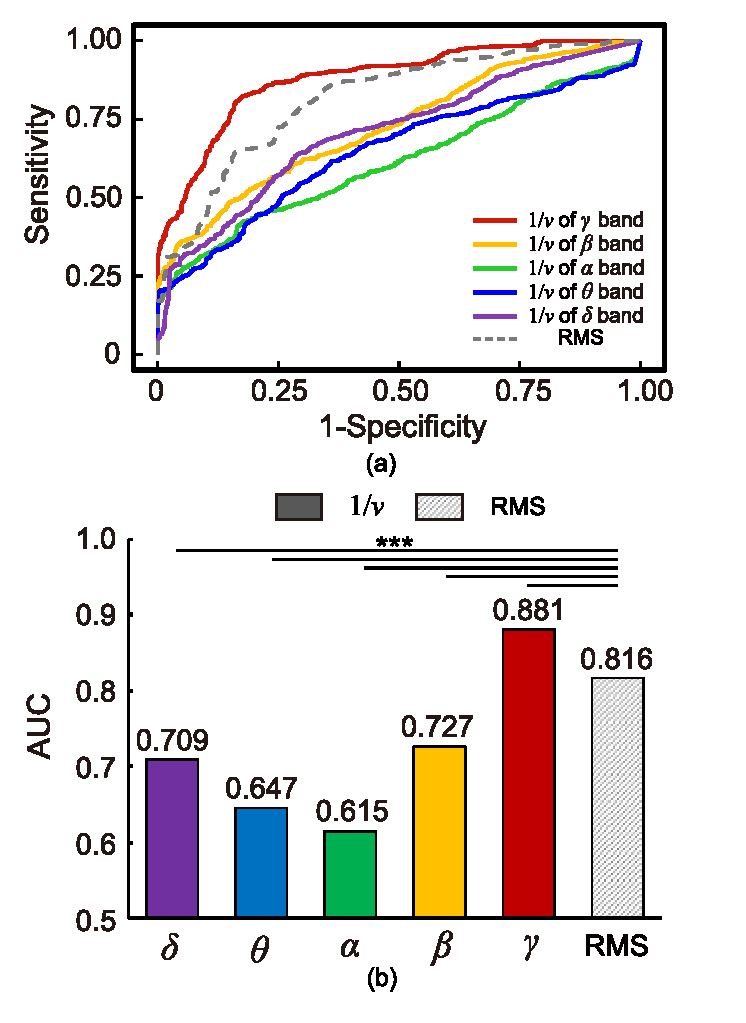
\includegraphics[width=0.9\hsize]{figure/ROC_rms_ver5.eps}
%\end{center}
\caption{Results of $1/\nu$ for each frequency band and RMS. (a) ROC curves. (b) AUCs. The pairwise comparisons between RMS and the others result based on the Delong's test for two correlated ROC curves with Holm adjustment are also shown (***: $p<0.001$).}
\label{fig:roc}
\end{figure}
%%%%%%%%%%%%%%%%%%%%%%%%%%%%%%%%

%%%%%%%%%%%%%%%%%%%%%%%%%%%%%%%%
%\begin{figure}[!t]
%\centering
%\includegraphics[width=0.95\hsize]{figure/window_w50.eps}
%\end{center}
%\caption{Results of AUCs for each frequency band by changing window length. }
%\label{fig:window}
%\end{figure}
%%%%%%%%%%%%%%%%%%%%%%%%%%%%%%%%

\section{Discussion}
%-------------------
%考察
%-------------------
シミュレーション実験において,
Fig. \ref{fig:sim_EEG}より,$\nu_0$の値が$\nu_0 = 5.0$から$\nu_0 = 13.0$に変更するにつれて波形の外れ値は頻出しなくなり,定常的な波形になっていることがわかる.これは,$\nu$が分布のガウス性を決定するパラメータであることから値が大きくなるにつれて分布がガウス分布に近づくことを表している.
また,${\psi_0}_{ii}$の値においては,${\psi_0}_{ii}=10.0$から${\psi_0}_{ii}=40.0$に変更するにつれて,生成データの振幅が大きくなっていることがわかる.これは,$\mathbf{\Psi}$の対角成分である$\psi_{ii}$は,各次元における脳波の分散スケールを特徴づけるパラメータであるためである.

Fig. \ref{fig:ES_param}より,$\nu$, $\mathbf{\Psi}$のAverage absolute percentage errorが$W$ = 100 sにおいておよそ2%程度になっており,正確に推定が行なえていることがわかる.しかし,窓幅を小さくすると,$W$ = 1 sにおいて$\nu$で最大約25\%,$\mathbf{\Psi}$で約35\%まで誤差率が上昇している.このことから精度は窓幅の長さに依存することがわかる.
また,次元数を増加させた場合,$\nu$においては,Average absolute percentage errorが減少しており,$\mathbf{\Psi}$においては一度減少し,再び増加するという傾向が確認された.
$\nu$は入力次元全体に対して一次元で定義されるパラメータである.そのため,次元数を大きくすることで推定対象となる実質的なサンプルサイズが増加し,Average absolute percentage errorが減少したと考えられる.
$\mathbf{\Psi}$に関しては,$\mathbf{\Psi} = \nu' \mathbf{\Psi}'$より,$\nu'$の推定精度の影響を受けるため,小さい次元数の場合,相乗的に誤差率が大きくなっていると考えられる.
一方,大きい次元数の場合,Average absolute percentage errorが増加していることがわかる.
これは行列の要素数が増加し,要素ごとの推定精度は変化せずとも,フロベニウスノルムを用いて計算を行なっているため,全体としてのAverage absolute percentage errorは大きくなったと考えられる.
以上のことから,窓幅を大きくすることで,$\nu$,$\mathbf{\Psi}$はより正確に推定を行なうことができ,次元数を大きくすることで$\nu$はより正確に,反対に$\mathbf{\Psi}$の推定精度は減少することがわかった.これらの結果より,international 10--20 electrode systemで用いられる電極数である19次元において,窓幅が5 s以上であれば,少なくとも10\%以下の誤差,特に$W$ = 15 sの場合は5\%程度の誤差で推定が行なえると考えられる.

脳波解析実験において,
Table \ref{table:BIC}より,各周波数帯域において,提案モデルのBICが最も最小となる回数が多いことがわかる.しかし,$\delta$帯域の場合,ガウスモデルのBICが最小となる割合が17.92\%であり,他の帯域より多くなることが確認された.これは,低周波帯域では,それぞれの窓幅内の分布形状が大きく異なってしまうことが原因であると考えられる.また,提案モデルのパラメータ数($k_t=382$)がガウスモデル($k_g=381$)よりも1大きいことからわずかな差でガウスモデルがより適したモデルであると判定されたと考えられる.ただし,その他の周波数帯域では,BICが最小となる回数が95\%以上であり,提案モデルが他モデルより脳波に適したモデルであることがわかる.これは,提案モデルのパラメータ$\nu$を変更させることで,外れ値が少ないガウスモデルと裾の重い分布となるコーシーモデル双方に適応できるためであると考えられる.
また,高周波帯域になるにつれて,提案モデルのBICが最小となる割合が増加している.これは,周波数特性に応じて脳波の分布も変化しており,信号の変化が速い高周波帯域の分布が提案モデルによく適合したためであると考えられる.

Fig. \ref{fig:Colormap}より,てんかん発作区間において特に高周波帯域の$1/\nu$が大きくなっていることがわかる.
この傾向は,全ての被験者に共通して確認することができた.このことから,提案法を用いることで,てんかん発作に伴う脳波の非ガウス性の変化を確率的変動として定量的に評価できていると考えられる.
しかしながら,Fig. \ref{fig:Colormap}(a)の220 s付近を見ると,てんかん発作以外の区間においても部分的な$1/\nu$の増加が認められた.これは,筋電位などの高周波帯域のアーティファクトにより確率的変動が大きくなったためであると考えられるため,専門医の知見に基づき,解析結果についてより詳細に検討していく必要がある.

Fig. \ref{fig:dens}より,全被験者の各帯域における$1/\nu$の分布を確認すると,非発作時の$1/\nu$は帯域によらず0.02--0.03の領域に分布していることがわかる.一方,発作時の$1/\nu$は非発作時よりも大きい値で分布しており,その傾向は高周波である$\gamma$帯域で最も顕著に表れていることがわかる.これは平均値の差の程度を表す効果量$g$の結果からも確認できる.$\gamma$帯域において大きな効果量が得られたことから,高周波帯域における$1/\nu$がてんかん発作時の特徴を最も反映していると考えられる.これは,てんかん発作に伴い脳波の高周波帯域が強い非ガウス性を示したことを意味している.てんかん発作時に脳波の高周波帯域である$\gamma$帯域の活動が活発になることは従来研究においても報告されている~\cite{Kobayashi2004,Kobayashi2009,Benedek2016}.その詳しいメカニズムはいまだ明らかにされていないものの,皮質と皮質下構造の間の複雑な相互作用に起因すると考えられている~\cite{Kobayashi2004}.この相互作用の異常によっててんかん発作時特有の断続的な振幅変化が生じ,結果として高周波帯域の非ガウス性が強調され$1/\nu$が増加した可能性がある.

Fig. \ref{fig:roc}(b)より,各帯域における$1/\nu$のAUCを確認したところ,高周波帯域である$\gamma$帯域で0.881と中程度ながら高い値が得られており,$\gamma$帯域の$1/\nu$が最も分類性能が高いことがわかる.また,従来の特徴量であるRMSと有意な差を確認したため,$\gamma$帯域の$1/\nu$は従来の特徴量以上の識別性能を有することが示された.振幅の絶対的な大きさであるRMSや振幅の情報をもつと考えられる$\mathbf{\Psi}$と,提案法から算出される$1/\nu$は脳波活動の異なる側面を捉えていると考えられるため,今後はこれらを組み合わせることでより高い識別性能を獲得できる可能性がある.

\section{Conclusion}
本稿では,尺度混合モデルを用いて多チャネル脳波のモデル化を行なった.
提案モデルにおいて,頭皮表面の多チャネル電極から計測された脳波を多変量ガウス分布,
そしてその分散共分散行列を逆ウィシャート分布に従う確率変数として扱うことで,てんかん発作に伴う脳波の確率的変動を評価可能であることを示した.
解析法では,脳波をフィルタバンクを用いて複数の周波数帯域に分解し,提案モデルに基づく推定を行なうことで,各周波数帯域における確率的変動を特徴づける指標を導入した.

シミュレーション実験では,各パラメータの推定精度を評価し,推定精度はサンプルサイズと次元数に依存して変化することを示した.
脳波解析実験においては,提案モデルが他モデルと比較して脳波に最も適したモデルであることを示し,$\gamma$帯域の提案指標$1/\nu$に着目することで従来の特徴量よりも高い精度(AUC=0.881)で分類可能であることを示唆した.

しかしながら,提案指標$1/\nu$は体動や体の硬直に起因する筋電図などのアーティファクトの影響を受けると考えられる.そのため,より実践的に提案法を展開するためには,これらのアーティファクトを検出・除去するようなアルゴリズムを導入する必要がある.また今後は,逆ウィシャート分布のもう一つのパラメータである$\mathbf{\Psi}$の評価やてんかん脳波以外の脳波への応用を検討する予定である.



\appendix[Equivalent calculation on MVSMM]
Equation (\ref{eq:eq6}) is equivalent to (\ref{eq:eq9}) as below:
\begin{align}
	p(\mathbf{x}_n) &= \int \mathrm{IG}(\tau_n;\nu'/2,\nu'/2) \mathcal{N}(\mathbf{x}_n|\tau_n \mathbf{\Psi}') \mathrm{d}{\tau_n} \nonumber\\
	&= \int \frac{\left(\frac{\nu'}{2}\right)^{\frac{\nu'}{2}}}{\Gamma \left(\frac{\nu'}{2}\right)} (\tau_n)^{-\frac{\nu'}{2}-1} \mathrm{exp} \left[-\frac{1}{\tau_n} \left(\frac{\nu'}{2} \right) \right] \nonumber\\
	&\quad\times\frac{1}{(2\pi)^{\frac{D}{2}}(\tau_n)^{\frac{D}{2}}|\mathbf{\Psi'}|^{\frac{1}{2}}} \mathrm{exp} \left[-\frac{1}{2}\mathbf{x}^\mathrm{T} (\tau_n\mathbf{\Psi'})^{-1} \mathbf{x}\right] \mathrm{d}{\tau_n} \nonumber\\
	&=\frac{1}{(2\pi)^{\frac{D}{2}}}\frac{\left(\frac{\nu'}{2}\right)^{\frac{\nu'}{2}}}{\Gamma \left(\frac{\nu'}{2}\right)}\frac{1}{|\mathbf{\Psi'}|^{\frac{1}{2}}} \nonumber\\
	\label{eq:20}
	&\quad\times \int (\tau_n)^{-\frac{\nu'+D}{2}-1} \mathrm{exp} \left[-\frac{1}{\tau_n} \left(\frac{\nu' + \Delta'}{2}\right) \right] \mathrm{d}{\tau_n}.
\end{align}
Multiply (\ref{eq:20}) of the equation by $\frac{\Gamma \left(\frac{\nu'+D}{2}\right)}{\left(\frac{\nu'+\Delta'}{2}\right)^{\frac{\nu'+D}{2}}} \times \frac{\left(\frac{\nu'+\Delta'}{2}\right)^{\frac{\nu'+D}{2}}}{\Gamma \left(\frac{\nu'+D}{2}\right)}$.
\begin{align}
	p(\mathbf{x}_n) &=\frac{1}{(2\pi)^{\frac{D}{2}}}\frac{\left(\frac{\nu'}{2}\right)^{\frac{\nu'}{2}}}{\Gamma \left(\frac{\nu'}{2}\right)}\frac{1}{|\mathbf{\Psi'}|^{\frac{1}{2}}} \frac{\Gamma \left(\frac{\nu'+D}{2}\right)}{\left(\frac{\nu'+\Delta'}{2}\right)^{\frac{\nu'+D}{2}}}\nonumber\\
	&\quad\times \int \frac{\left(\frac{\nu'+\Delta'}{2}\right)^{\frac{\nu'+D}{2}}}{\Gamma \left(\frac{\nu'+D}{2}\right)} (\tau_n)^{-\frac{\nu'+D}{2}-1} \nonumber\\
	&\quad\times \mathrm{exp} \left[-\frac{1}{\tau_n} \left(\frac{\nu' + \Delta'}{2}\right) \right] \mathrm{d}{\tau_n} \nonumber\\
	&=\frac{1}{(2\pi)^{\frac{D}{2}}}\frac{\left(\frac{\nu'}{2}\right)^{\frac{\nu'}{2}}}{\Gamma \left(\frac{\nu'}{2}\right)}\frac{1}{|\mathbf{\Psi'}|^{\frac{1}{2}}} \frac{\Gamma \left(\frac{\nu'+D}{2}\right)}{\left(\frac{\nu'+\Delta'}{2}\right)^{\frac{\nu'+D}{2}}}\nonumber\\
	\label{eq:21}
	&\quad\times \int \mathrm{IG}(\tau_n;\frac{\nu'+D}{2},\frac{\nu'+\Delta'}{2}) \mathrm{d}{\tau_n},
\end{align}
where the integral of probability density function over the entire space is equal to 1 (\ref{eq:22}).
\begin{align}
\label{eq:22}
\int \mathrm{IG}(\tau_n;\frac{\nu'+D}{2},\frac{\nu'+\Delta'}{2}) \mathrm{d}{\tau_n}=1.
\end{align}
From (\ref{eq:21}) and (\ref{eq:22}), $p(\mathbf{x}_n)$ can be derived as follows:
\begin{align}
	p(\mathbf{x}_n) &= \frac{\Gamma(\frac{\nu'+D}{2})}{\Gamma(\frac{\nu'}{2})} \frac{|{\bm \Psi'}|^{-\frac{1}{2}}}{\left(\pi \nu' \right)^{\frac{D}{2}}} \left(1+\frac{\Delta '}{\nu '} \right)^{-\frac{\nu'+D}{2}}.
\end{align}

% if have a single appendix:
%\appendix[Proof of the Zonklar Equations]
% or
%\appendix  % for no appendix heading
% do not use \section anymore after \appendix, only \section*
% is possibly needed

% use appendices with more than one appendix
% then use \section to start each appendix
% you must declare a \section before using any
% \subsection or using \label (\appendices by itself
% starts a section numbered zero.)
%



% use section* for acknowledgment
%\section*{Acknowledgment}


%The authors would like to thank...


% Can use something like this to put references on a page
% by themselves when using endfloat and the captionsoff option.
\ifCLASSOPTIONcaptionsoff
  \newpage
\fi



% trigger a \newpage just before the given reference
% number - used to balance the columns on the last page
% adjust value as needed - may need to be readjusted if
% the document is modified later
%\IEEEtriggeratref{8}
% The "triggered" command can be changed if desired:
%\IEEEtriggercmd{\enlargethispage{-5in}}

% references section

% can use a bibliography generated by BibTeX as a .bbl file
% BibTeX documentation can be easily obtained at:
% http://mirror.ctan.org/biblio/bibtex/contrib/doc/
% The IEEEtran BibTeX style support page is at:
% http://www.michaelshell.org/tex/ieeetran/bibtex/
%\bibliographystyle{IEEEtran}
% argument is your BibTeX string definitions and bibliography database(s)
%\bibliography{IEEEabrv,../bib/paper}
%
% <OR> manually copy in the resultant .bbl file
% set second argument of \begin to the number of references
% (used to reserve space for the reference number labels box)

\bibliographystyle{IEEEtran}
\bibliography{ref.bib}




% if have a single appendix:
%\appendix[Proof of the Zonklar Equations]
% or
%\appendix  % for no appendix heading
% do not use \section anymore after \appendix, only \section*
% is possibly needed

% use appendices with more than one appendix
% then use \section to start each appendix
% you must declare a \section before using any
% \subsection or using \label (\appendices by itself
% starts a section numbered zero.)
%




% You can push biographies down or up by placing
% a \vfill before or after them. The appropriate
% use of \vfill depends on what kind of text is
% on the last page and whether or not the columns
% are being equalized.

%\vfill

% Can be used to pull up biographies so that the bottom of the last one
% is flush with the other column.
%\enlargethispage{-5in}



% that's all folks
\end{document}
